% Drawing 152/01-4 -- folder 152, batch 01, archive page 10 (PDF page 11).
% Transcription: au bas du feuillet, à gauche : un disque dont le bord, épaissi par endroits, porte une vingtaine de petits traits et de points marqués, et à l'intérieur duquel sont tracées huit cordes courbes qui ne se rencontrent pas : une longue corde du haut vers le bas, deux cordes emboîtées en haut à droite, une longue corde à droite, une corde à gauche, une petite à droite, deux petites en bas.
% Kind: disc with marked boundary points and non-crossing chords. Method 2 (schematic redraw from the facsimile). Status: partial.
% Notes: The disc (an ellipse fitted to his outline), about twenty marks on the rim (short radial ticks, heavier at the left, at the upper right and at the right, where he went over them), and eight curved chords inside, none crossing another, each ending on the rim (ends computed on the outline): (1) at the left, from the upper left to the left; (2) the long one from the top down to the lower right of the bottom; (3) and (4) two nested arches at the upper right, starting beside the top of (2) and ending at the two marks of the upper right; (5) a long one from the outer end of (4) down the right side to the lower right; (6) a small bump on the right rim; (7) a low arch at the bottom left; (8) a small arch at the bottom. Disagreement with the note of the transcription, which says « trois cordes »: eight are counted. Still differs: the exact number of marks on the rim (some are doubled or blotted), and which mark each chord end meets: the ends are put on the rim where the strokes arrive, without being snapped to a mark. Whether (4) and (5) share their end at the upper right, as drawn, is a reading. Redrawn 2026-11-12 (issue 128): to check again.
% Coordinates: 1 unit = 1 mm = 1/100 of the crop width (bbox in page fractions: [0.11, 0.535, 0.43, 0.765]).
% Redrawn by Claude (claude-fable-5-2), issue #128, 2026-11-12; not checked by a human; not compiled (no TeX in the session).
% Rights: reproduces part of the work -- behind RENDER_TRANSCRIPTS, never published by itself.
\documentclass[tikz,border=3pt]{standalone}
\usepackage{amsmath,amssymb}
\usetikzlibrary{patterns,arrows.meta}
\tikzset{pencil/.style={black!45}, struck/.style={black!35}, mpt/.style={circle,draw,inner sep=1.3pt}, pt/.style={circle,fill,inner sep=0.9pt}, opt/.style={circle,draw,fill=white,inner sep=1.1pt}}
\begin{document}
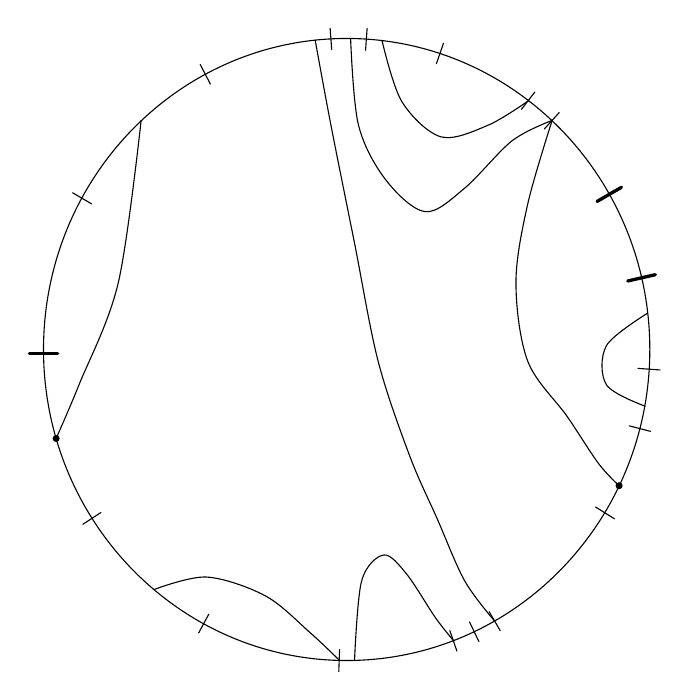
\begin{tikzpicture}[x=1mm,y=1mm,line cap=round,line join=round,font=\scriptsize]
\draw (49,-53.5) ellipse[x radius=38.5, y radius=39.5];
\draw (31.7,-19.8) -- (30.4,-17.3);
\draw (47.1,-15.4) -- (46.9,-12.7);
\draw (51.4,-15.5) -- (51.6,-12.7);
\draw (60.4,-17.2) -- (61.3,-14.6);
\draw (71.2,-23) -- (72.9,-20.8);
\draw (74.1,-25.5) -- (76,-23.4);
\draw (86,-55.9) -- (88.8,-56.1);
\draw (84.9,-63.2) -- (87.6,-63.9);
\draw (80.6,-73.5) -- (83,-75);
\draw (17.8,-74.2) -- (15.5,-75.7);
\draw (16.6,-35) -- (14.2,-33.6);
\draw (31.5,-87.1) -- (30.2,-89.5);
\draw (48.1,-91.6) -- (48,-94.4);
\draw (62.1,-89.2) -- (63,-91.8);
\draw (64.6,-88.1) -- (65.8,-90.6);
\draw (67.1,-86.8) -- (68.5,-89.2);
\draw[very thick] (80.8,-34.7) -- (83.9,-32.9);
\draw[very thick] (84.7,-44.8) -- (88.2,-44);
\draw[very thick] (12.3,-54) -- (8.7,-54);
\node[pt] at (83.6,-70.8) {};
\node[pt] at (12.1,-64.8) {};
\draw plot[smooth, tension=0.55] coordinates {(22.9,-24.4) (20,-45) (15,-58) (12.1,-64.8)};
\draw plot[smooth, tension=0.55] coordinates {(45,-14.2) (47,-25) (50,-40) (53,-55) (57,-67) (60.5,-75) (64,-82.9) (67.8,-88)};
\draw plot[smooth, tension=0.55] coordinates {(53.5,-14.3) (56,-22) (61,-26.5) (67,-25) (72.1,-21.9)};
\draw plot[smooth, tension=0.55] coordinates {(49.5,-14) (50.5,-25) (54,-32) (59,-36) (64,-33) (70,-27) (75.1,-24.4)};
\draw plot[smooth, tension=0.55] coordinates {(75.1,-24.4) (72,-35) (70.5,-45) (72,-55) (77,-62) (81,-68) (83.6,-70.8)};
\draw plot[smooth, tension=0.55] coordinates {(87.2,-48.9) (82,-53) (82,-58) (86.9,-60.7)};
\draw plot[smooth, tension=0.55] coordinates {(24.5,-84) (31.2,-82.4) (38.7,-84.8) (44.4,-89.5) (48.1,-93)};
\draw plot[smooth, tension=0.55] coordinates {(50,-93) (50.9,-82.9) (53.7,-79.6) (56.6,-82) (60.3,-87.6) (62.6,-90.5)};
\end{tikzpicture}
\end{document}
